\documentclass[oneside,a4paper,english,links]{amca}
%
\usepackage{graphicx}
\usepackage{amsmath,amsfonts}

\title{REAL TIME DIRECT VOLUME RENDERING OF BREAD CRUMBS}

\author[a]{Rodrigo Baravalle}
\author[b]{Leonardo Scandolo}
\author[c]{Claudio Delrieux}
\author[d]{Cristian G. Bauza}
%
\affil[a]{Laboratory for System Dynamics and Signal Processing, FCEIA, Rosario National University, CIFASIS-CONICET,
  Ocampo y Esmeralda, S2000EZP~Rosario, Argentina,
  baravalle@cifasis-conicet.gov.ar, \url{http://www.cifasis-conicet.gov.ar/grupo4.html}}
%
\affil[b]{Computer Science Department, FCEIA, Rosario National University,
  Pellegrini 250, 2000~Rosario, Argentina,
  leonardo@fceia.unr.edu.ar, \url{http://web.fceia.unr.edu.ar/es/institucional/escuelas/118-departamento-ciencias-de-la-computacion-ecen.html}}

\affil[c]{Department of Electrical Engineering and Computers, Universidad Nacional del Sur - IIIE-CONICET,
  Col\'on 80, 8000FTN~Bah\'ia Blanca, Argentina,
  cad@uns.edu.ar, \url{http://www.ingelec.uns.edu.ar/}}

\affil[d]{Research Institute PLADEMA- Faculty of Exact Sciences - Universidad Nacional del Centro,
  Paraje Arroyo Seco, (B7001BBO) Tandil, Buenos Aires, Argentina
  crgarcia@exa.unicen.edu.ar, \url{http://www.exa.unicen.edu.ar/es/d_investigacion/inst_pladema/index.html}}


%% NOTE: IF ALL AUTHORS BELONG TO THE SAME AFFILIATION
%% USE THE `\voidaffil' MACRO FOR THE AFFILIATION CODE.
%% Example:
%% \author[\voidaffil]{First A. Author}
%% \author[\voidaffil]{Second B. Author}
%% \author[\voidaffil]{Third C. Author}
%% \author[\voidaffil]{Fourth D. Author}
%% %
%% \affil[\voidaffil]{Grupo de Mec\'anica Computacional,
%% Universidad Nacional de Villa Carolina,
%% Los Alerces 3492, 4200 Villa Carolina, Argentina,
%% gmc@uncarolina.edu.ar, http://www.uncarolina.edu.ar/gmc}

\begin{document}
\vspace{3cm}

\maketitle

%% To set PDF METADATA: uncomment and replace fields in
%% UPPERCASE with appropriate values. 
%% 
%% \hypersetup{
%%   pdfauthor={AUTHORS},
%%   pdfkeywords={KEYWORDS},
%%   pdftitle={TITLE}
%% }
%%
%% For instance
%% \hypersetup{
%%   pdfauthor={Sponge B. and Star P.},
%%   pdfkeywords={multiphase flow, air-liquid mixtures},
%%   pdftitle={A new model for multi-phase flow}
%% }
%%
%% NOTE: To set the metadata is recommended but not absolutely
%% neccesary. 
%% This was done before with the \pdfinfo command,
%% but according to this post:
%% http://de.nntp2http.com/comp/text/tex/2008/12/5358fd061de9703a781885a5dcf98364.html
%% if `hyperref' is used, then you must use \hypersetup{} not \pdfinfo{}

\begin{keywords}
  Direct Volume Rendering, Bread Crumb, Real Time.
\end{keywords}

\begin{abstract}
  Photo-realistic modelling and rendering of materials with complex internal structure poses a hard challenge in the Computer Graphics community. In particular, bread crumbs consist of a complex translucent material with a porous structure that presents different details at different scales. Realistic bread crumb rendering involves several light phenomena such as subsurface scattering, self-shadowing, self-occlusion, reflectance, and absorption. Current approaches to realistic recreate these phenomena use an  approximation of the rendering equation ({\em i.e.}, they account for global illumination as in ray and path tracing). Nevertheless, they are computationally expensive and generally require a detailed bread crumb mesh.

  State of the art techniques for bread crumb rendering set up a complex capture procedure, in which the light reflecting off the material is sampled at different angles. The methods use that information to reconstruct a material model. While this solution accounts for several desired properties of this material, it presents several drawbacks which makes difficult its practical applications: high computational costs, complex capture procedures, and poor image variability.

  In this work we propose to study and implement a GPU based direct volume rendering on a scalar field to represent the internal structure of a bread crumb, without requiring any intermediate steps. The images obtained show promising results at interactive and real time frame rates. We represent the crumb as a 3D scalar field, computing it in two steps. The first uses a particle-system based generation procedure, and the second uses dynamic systems to evolve the particles mimicking the bread making process.
\end{abstract}

\section{INTRODUCTION}

The computer graphics community has considered challenging to render the appearance of  baked materials, such as
pizzas and cookies, due to
the complex interaction of light outside and inside the
material. Computational costs of these
physical simulations made its rendering impractical in areas with high
interaction with the final user. The exponential growth in
computing power, based on the massively parallel design of modern
graphics cards \citep{Yeo09,Harris06}, has made it possible to
simulate some light phenomena at acceptable computational rates, but
the field is still a subject of research \citep{Voglsam2013}.

The geometry of these materials represents an additional challenge. These porous structures are the
result of complex mechanisms involving physical deformations and
chemical reactions. Bread making involves two different
processes: proofing and baking. Proofing accounts for
chemical reactions between the living yeast and the dough. The yeast
produces $CO_{2}$ making bubbles in the dough
\citep{Shah1998}. In the baking process \citep{Mondal2008},
temperature changes these shapes in several ways \citep{Scanlon2001},
giving bread its final internal structure. The literature reports a few attempts to
synthesise a model of the resulting geometrical structure \citep{VanDyck2014,Cho2007}, but the process is an artistic design or its variability is limited to the amount of captures
made. In this work we propose to employ dynamical systems
\citep{Strogatz2001} in order to evolve particle systems
\citep{Reeves83}, which we have previously designed
\citep{Baravalle2011}, trying to mimic the bread making process
(proofing and baking). Differential equations govern many complex processes, such as weather and
fluids, describing their
dynamics and appearance. We employ this idea
to describe bubble growth in bread. This process produces a
structure similar to bubbles growing inside a fluid. Other approaches compute
texel values using algebraic functions without requiring to
store a 3D texture in memory \citep{Perlin1989}, but they
are not adequate since bubble distributions are difficult to
model statistically.

The mechanism for rendering the internal constitution of these materials largely depends
on the data structure chosen for its representation. Triangular
meshes should be computed from voxel data, using
techniques such as marching cubes \citep{Lorensen1987}. Nevertheless
the porous bread structure makes it a non-trivial task, and it
could be high memory demanding.

The presence of mesostructures (surface bubbles) makes bread a quasi homogeneous material \citep{Tong2005}. Surface representations
of this material are not adequate since it presents visible structures on it: typical solutions such as
Bidirectional Reflectance Distribution Functions (BRDF)
\citep{Kurt2009} and Bidirectional Surface Scattering Reflectance
Distribution Functions (BSSRDF) \citep{Donner2009} are not completely
adequate. A material model \citep{Tong2005} solves these limitations, but the associated drawbacks (complex capture procedure
involved, computational costs, poor image and structure variability),
made its widespread application very difficult.

In this paper we propose to apply Direct Volume Rendering (DVR)
\citep{Levoy1988,Kruger2003, Kratz2006} on a scalar field to render
the bread crumb structure. DVR applies ray marching through a volume
accumulating different properties for each pixel. The method does not
use intermediate structures, simplifying the modelling
process. In addition, the bread crumb shape can be defined in
real time on the GPU, with the possibility of performing arbitrary cuts and
slices of the 3D structure in real time. Also, the
bread crust can be easily defined along with its own properties like
colour and translucency, using transfer functions. We obtain satisfactory results at real time rates.

Authors organise this paper as follows. In section 2 we introduce the theory of
particle systems, dynamical systems and DVR. In section
3 we show and discuss the results. In section 4 we summarise the conclusions,
as well as possible future works.

\section{MATERIALS AND METHODS}

\subsection{Particle systems}

Early approaches in computer graphics represented objects using Euclidean geometry. In other words, combining points, lines, surfaces, and other simple primitives. Nevertheless, it is difficult to capture details of natural structures with this approach. Other approaches such as fractal geometry \citep{Mandelbrot83} describes natural phenomena more adequately.

Particle systems \citep{Reeves83} deals with phenomena which have no well defined surface, like water,
smoke, and fire. Particle systems are composed of entities called {\em
  particles} that evolve properties over time. For instance, the method can render fireworks defining a common space position, and after
each time step modifying each particle position following a parabola, with different
particles following slightly different parabolas. The method obtains an animation. Particle systems renders fire and other effects modifying properties as colour, size and direction. Particles can also affect each other.

In a previous work \citep{Baravalle2011}, we employed particle systems for texture synthesis. Each particle had an initial random position in an image, and evolved avoiding other particles. We obtained adequate results for wood and painting textures. The growing functions were random, vertical, horizontal and diagonal. We propose to emulate the bread making process by extending it into space, using a system of differential equations to control the particles growth. The result is a 3D texture representing this material. 

\subsubsection{Modelling algorithm}
This algorithm produces a geometry for rendering. Therefore, instead of delivering the colour of a particular space position it will generate a scalar field composed of $0$s and $1$s ($0$: air, $1$: mass). This representation is adequate for DVR.

The system consists of a set of particles $P$, 

\begin{equation}
  P = \{p_{1}, ... , p_{n}\}, n  \in \mathbb{N},
\end{equation}

\noindent a lattice $L_{N\times N \times N}, N \in \mathbb{N} $ (initially $L_{xyz}=1$) of mass and air, and a lattice $L2_{N\times N \times N}$, (initially $L2_{xyz}=-1$), of positions and particle ownership ($i$ if the lattice element belongs to the contour or interior of the particle $i$).

Each element in $P$ has the following properties:

\begin{equation}
  p_{i} = \{O_{i}, C_{i}\}, 1 \le i \le n,
\end{equation}

\noindent where:

\begin{itemize}
\item $O_{i} = \{o_{1}, ... , o_{n_{i}}\}$: (Occupied) vector (set) of occupied positions by the particle in $L$.

\item $C_{i} = \{c_{1}, ... , c_{m_{i}}\}$: (Contour) vector (set) of positions representing the particle {\em contour} in $L$. The vector $O$ represents the positions affected by the particle, and the contour $C$ ensure avoidance with other particles.
\end{itemize}

The algorithm works as follows. When $t = 0$, a set of particles take random lattice positions. Each particle adds its position to $O$ and the surrounding positions to $C$. Then, for each $t$, each particle chooses a position on its contour. If the position lies in the contour of any other particle ($L2_{position} <> i$ and $L2_{position} > -1$), it is discarded and the process selects another contour position. If that position is free ($L2_{position} = i$ or $L2_{position} = -1$), the particle adds the position to its $O$ and updates its contour $C$ and the lattices. If the contour vector is empty, the particle {\em dies}, since it cannot grow anymore in the simulation.

Termination of the algorithm is possible at any $t$. The user can stop at a particular event, for instance, when the $L2$ lattice is full ($L2_{xyz} <> -1$ in any lattice position), since no progress can be made.

The method produces different structures varying the contour size (see Fig.~\ref{fg:fig1}). The image shows 2D output examples (for better understanding) of random growing particles. The contour size determines the white region among particles (mass) (the {\em width} of the white area). Resulting images seem to form voronoi-like patterns.


\begin{figure*}[htb!]
  \centerline{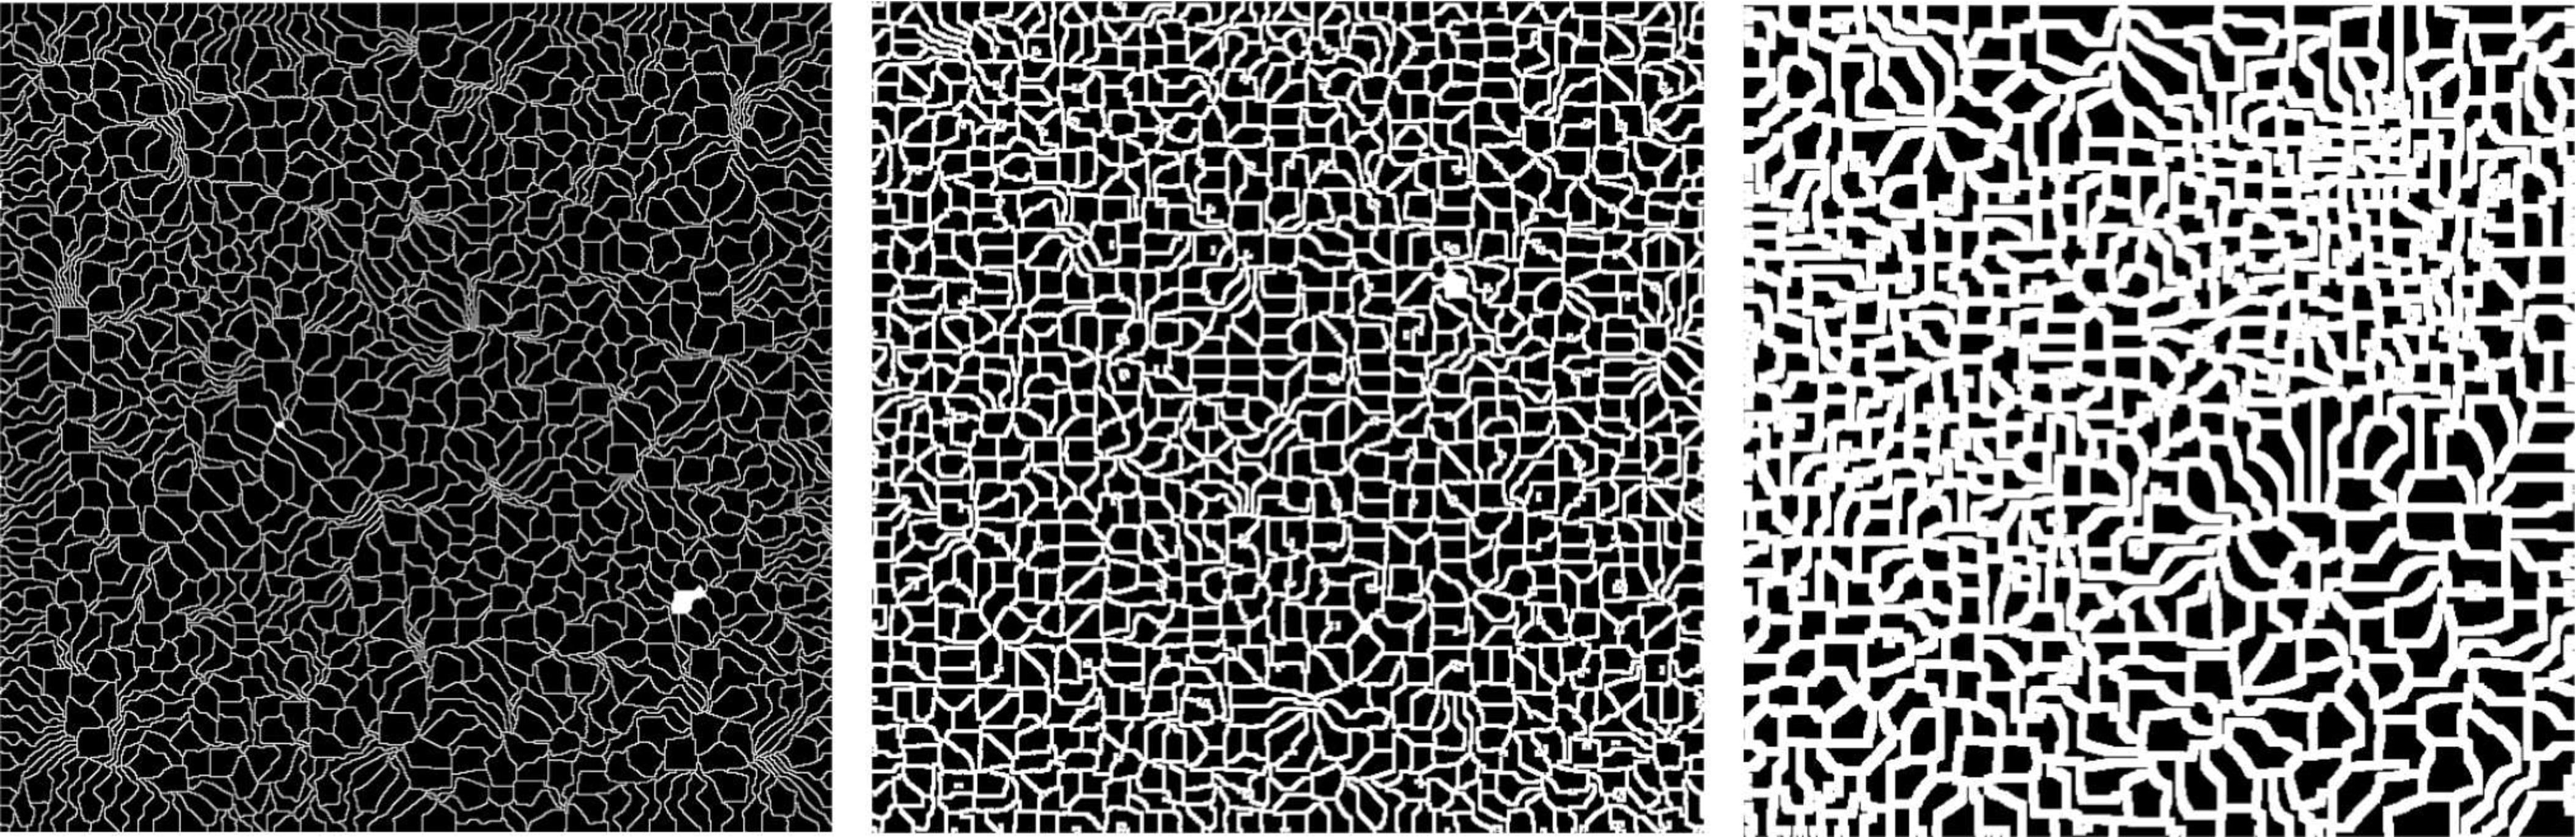
\includegraphics[scale=0.22]{fig1.pdf}}
  \caption{Different values for the contour parameter. Left: contour = 1, middle: contour = 2, right: contour = 4.}
  \label{fg:fig1}
\end{figure*}

The algorithm outputs the $L$ lattice. Next section establishes the system employed to evolve the particles over time.

\subsection{Dynamical systems}

Differential Equations manages the
difficulty (or impossibility) of finding analytical equations for
dynamical processes \citep{Strogatz2001}. Studies model dynamical phenomena by defining differential equations representing its behaviour. They simulate the evolution of the system and derive approximate solutions. Dynamical systems deals with processes such as economics, heat transfer, and fluids. With the development of computers, the field obtained insight into areas which were impossible before, such as Fractals \citep{Mandelbrot83}
and Chaos.

Mathematicians use numerical approximations to solve dynamical systems. The complexity of the problem and the number of equations involved changes its computational costs. We propose to employ a sub field of differential equations, Ordinary Differential Equations (ODE), for the purposes of this work. In ODEs, time is the only independent variable.

ODEs can be represented using the following set of equations:
\begin{equation} \label{eq:simple}  
  \begin{aligned}
    \dot{x_{1}} = f_{1}(x_{1},\ldots,x_{n}),\\
    \ldots\\
    \dot{x_{n}} = f_{n}(x_{1},\ldots,x_{n}),
  \end{aligned}
\end{equation}

\noindent where $\dot{x_{i}}$ represents the derivative of $x_{i}$ with respect
to $t$. The variables $x_{i}$ and the functions $f_{i}$
differ for each problem. In this work, each variable represents a
Cartesian coordinate in space, {\em i.e.,} $x_{1}$ is $x$, $x_{2}$ is
$y$ and $x_{3}$ is $z$ and we will define the set of $f_{i}$ to capture the bread crumb structure. The next section shows how these
systems can describe the evolution of a particle system.

\subsection{Particle evolution using dynamical systems}

Human perception can detect patterns in bread crumb structure (see
Fig.~\ref{fg:fig2}). First, bubble shape tends
to follow the crust shape. This is not casual, since temperature in
baking affects the bubbles' shape \citep{Scanlon2001}, stretching
them following its walls. Also, the entire
structure has a fluid-like appearance. Indeed, this is the case in
early stages of the baking process. At some point, the viscosity
of the dough decreases and the bubbles stop growing and
coalescing.

\begin{figure*}[htb!]
  \centerline{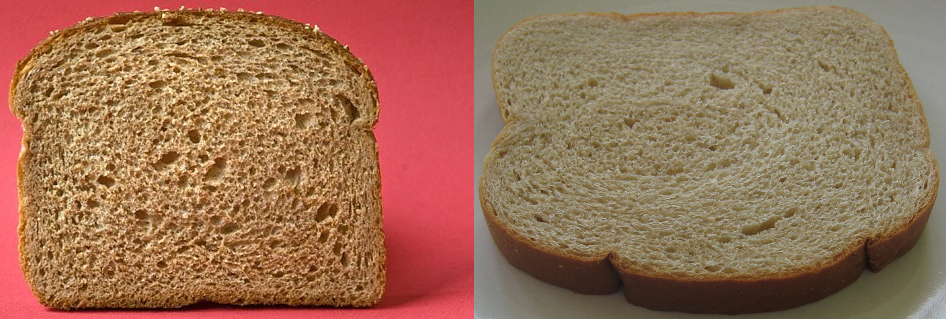
\includegraphics[scale=0.45]{fig2}}
  \caption{Images of real bread slices}
  \label{fg:fig2}
\end{figure*}

Dynamical systems produce natural shapes. If the domain is an image, the system outputs circles and spirals (see
Fig.~\ref{fg:fig3}). Three different set of equations
describe each image dynamics. For instance, the following set of equations produce the left
image:

\begin{equation} \label{eq:simple}  
  \begin{aligned}
    \dot{x} &= x^{2}-y^{2}+1,\\
    \dot{y} &= 2xy+1.
  \end{aligned}
\end{equation}


\begin{figure*}[htb!]
  \centerline{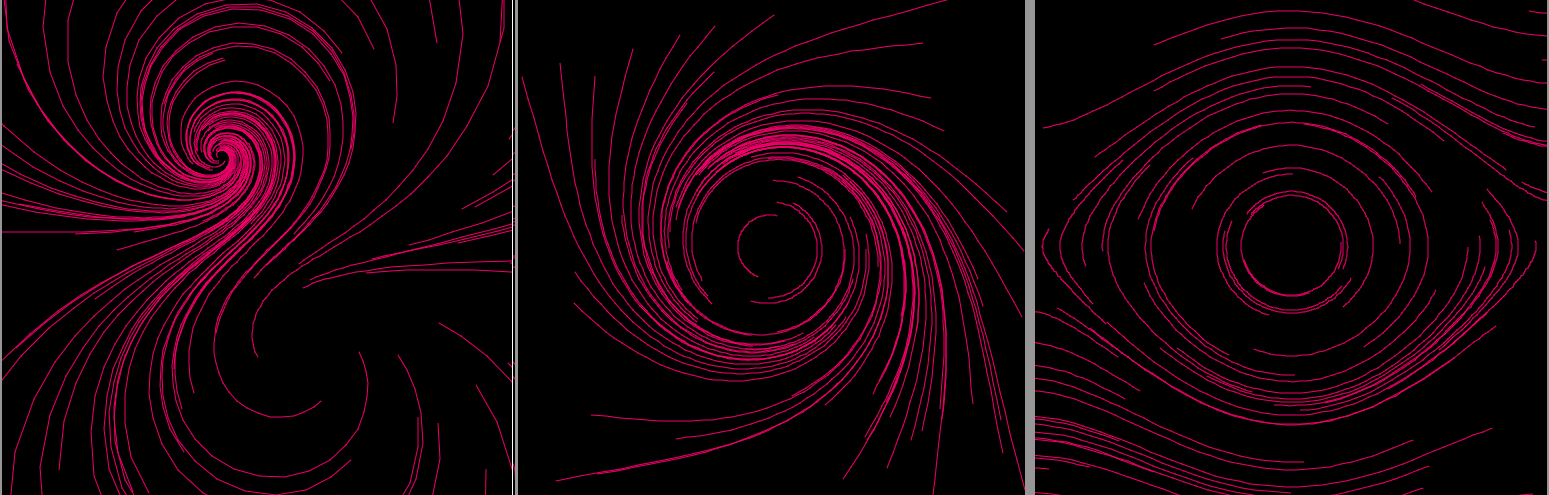
\includegraphics[scale=0.28]{fig3}}
  \caption{Dynamical systems in the plane.}
  \label{fg:fig3}
\end{figure*}


We chose random positions in the examples, and then we solve the system at each time step using a fourth order Runge-Kutta solver, determining the new trajectory direction. In the left image, an {\em attractor} attracts positions in the left-upper quadrant. A set of points can form an attractor, as in the right image. In this image trajectories follow circles and other shapes (the entire shape is an attractor).

Particles that follows trajectories produce patterns in the plane or space. In order for a particle to follow a trajectory, we solve the dynamical system at the current particle position, and we choose the contour position which best approximates that solution is chosen for growing. The dynamical system defines a vector field for the particles.

When we set the particles' growing directio to follow this vector field, we deform bubbles similarly to the dynamical system trajectories (see Fig.~\ref{fg:fig4}). In the
images, from left to right, we decrement the trajectories' {\em randomness}. The parameter randomness set to $0.1$ produces the right image, meaning
we force bubbles to follow the dynamical system
trajectories, with a probability of 0.9. We define this probability as
$1-randomness$, with $0 \leq randomness \leq 1$. The dynamical system
is the same as the right image in Fig.~\ref{fg:fig3}.  The
patterns are adequate for use not only in bread images, but also
cakes, and other baked foods, varying the randomness
parameter. Different useful structures can be defined by different set of equations and different parameters for the
particle systems (lifetime of particles, randomness).


\begin{figure*}[htb!]
  \centerline{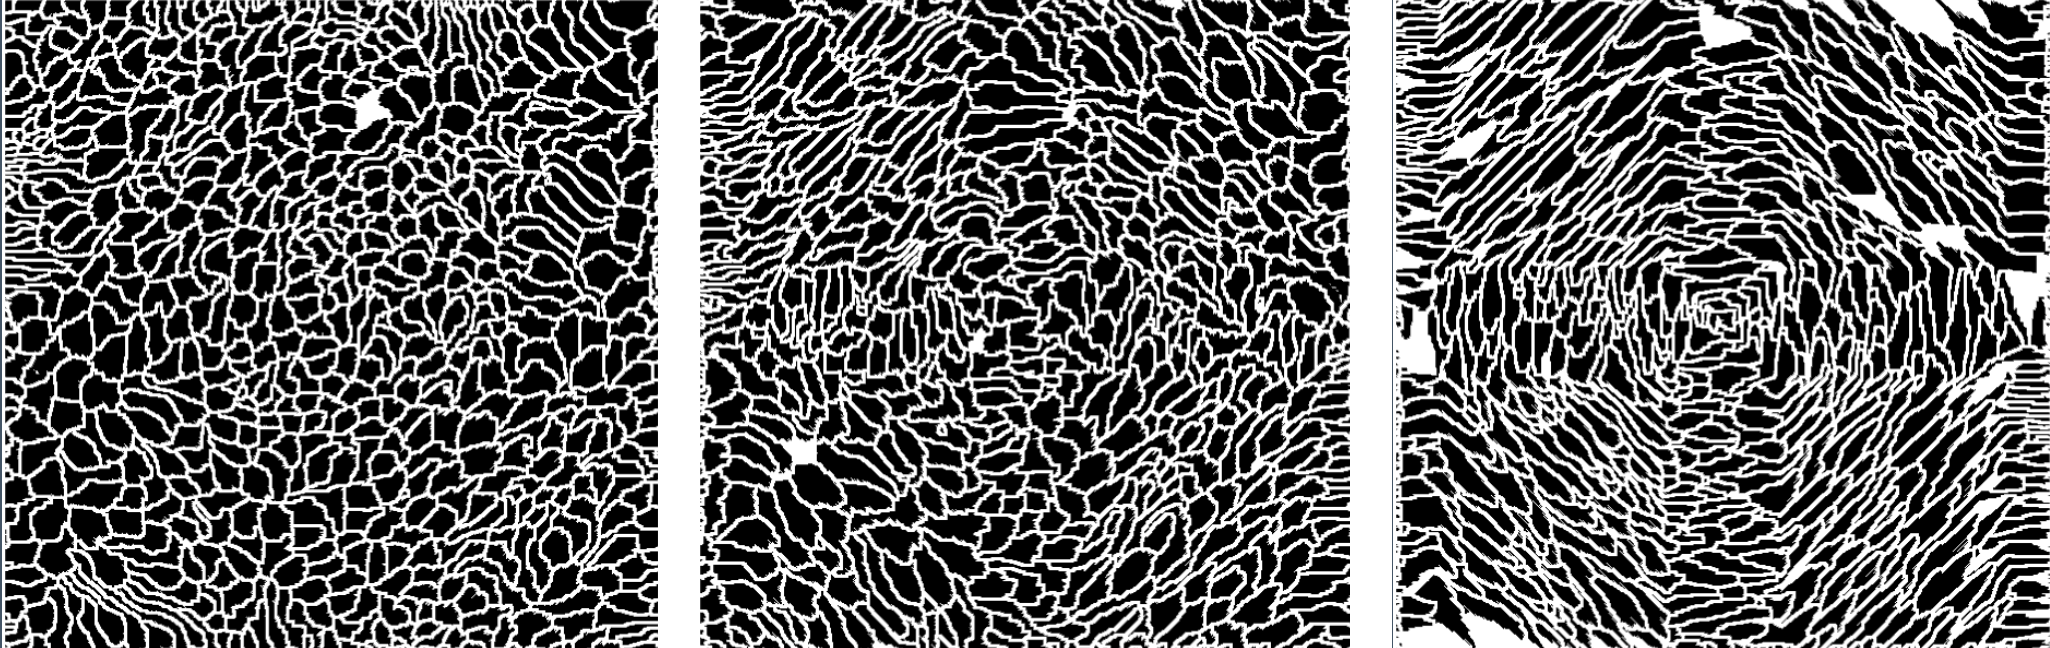
\includegraphics[scale=0.21]{fig4}}
  \caption{Dynamical systems affecting particle systems. Effect of the randomness parameter. From left to right, randomness: 0.3,0.2,0.1 respectively. }
  \label{fg:fig4}
\end{figure*}

The next section shows how these evolved particles can be rendered.

\subsection{Rendering algorithm}

In this section, the theory and implementation of the DVR algorithm used in this work is exposed.

\subsubsection{Direct volume rendering}

The technique of direct volume rendering attempts to provide a
2-dimensional representation of a volume defined by a discrete
3-dimensional density function. Rays are casted from the point of view
of a camera in a virtual scene and the density function is used to
compute the amount of light that the camera receives from the
direction of that ray. This is done by sampling the density function
along the ray in order to approximate the effect of different light
phenomena such as extinction, transmittance and scattering among
others. The lighting information gathered from these rays is then
used to compute the colour of the pixels in the final image.

Radiance is the amount of light that passes, or is emitted, from a
point and falls within a given solid angle. In the context of DVR, the
media that the rays traverse are taken as emissive, so when inspecting
the amount of light received for a given ray, what we are really doing
is approximating the radiance received from a distant point along the
direction of the ray. The radiance value is approximated by the
addition of the background radiance and the radiance emitted by the
media along the direction of the ray \citep{Kratz2006} : 

\begin{equation} \label{eq:general_radiance}  
  L(p_n) = L_b + \int_{p_0}^{p_n} \frac{\partial L(t)}{\partial p} \, dt,
\end{equation}

\noindent where $L_b$ is the background radiance, $p_0$ and $p_n$ are the
closest and furthest visible points along the ray direction,
respectively, $L(t)$ is the radiance sampled at point $t$, and
$\partial p$ is the distance between sampled points. For the purposes
of computing $L(p_n)$, the integral is approximated by a sum.

Extinction is the loss of photons in a ray shaft due to absorption in
the participating media and scattering to other directions. Some of
the photons will collide with the particles in the
surrounding media and be absorbed and transformed to energy, mostly
heat. Others will bounce and move along other directions. This is
approximated by using an absorption coefficient for the media, $k_a$
and a scattering coefficient $k_s$. If the scattering effect is
neglected, the formula for the amount of radiance absorbed over a
ray segment is:

\begin{equation} \label{eq:radiance_absorption}  
    L_b \ \displaystyle e^{-\int_{p_0}^{p_n} k_a(t) \, dt}.
\end{equation}

The value $\int_{p_i}^{p_j} k_a(t) \, dt$ is called the
absorption coefficient and referred to as $\tau_{(p_i, p_j)}$.

Transmittance is a complementary concept to extinction, and describes
the amount of light that passes through a media in a given
direction. The value of transmittance along two points $p_i$ and $p_j$
is:

\begin{equation} \label{eq:general_radiance}  
  T(p_i,p_j) = e^{-\tau_{(p_i, p_j)}}.
\end{equation}

If light emission is assumed to be a constant term ($\rho$) for
every point in the volume, our initial radiance estimate becomes:

\begin{equation} \label{eq:ray_radiance}  
  L(p_n) = L_b \ e^{-\tau(p_0, p_n)} + \int_{p_0}^{p_n} \rho \ e^{-\tau(t,p_n)} \, dt.
\end{equation}

This means that the radiance along points $p_0$ and
$p_n$ is the remaining background radiance after attenuation plus the
emission at every point in the ray, also attenuated.

DVR defines a volume inside which to sample a density function at
regular intervals and uses that information to approximate the
transmittance along those points and compute the amount of light
reaching the camera along the direction of a ray. The integral sum is
replaced by a discrete sum over the length of the ray that intersects
the volume.

Other effects can be accounted for, which augment the fidelity of the
final image, as well as the computing cost of the technique. Some of
these effects are phase, incidental scattering, and
out-scattering. Since the goal of this work is to achieve real time
frame rates, the basis of our rendering algorithm uses the simplified
transmittance only model.

\subsubsection{Implementation}

\paragraph{Overview}

In order to test the particle system used to describe the structure of
the bread, a demo application was created\footnote{available at
  \emph{\url{https://www.github.com/rbaravalle/Pysys}}} that uses the particle
system described to generate a volume texture. This volume texture is
then used to shade a cube with a DVR based shader. This demo shows
that the proposed method is compatible with current
rasterization-based real-time GPU rendering pipelines, providing a
realistic looking material, as well as shadow-map based real-time
shadows. This means that the material techniques proposed in this
article  can easily be integrated into any shader-based 3D engine with
minimal modifications.

\paragraph{Details}

The mesh defined for the model employing our DVR-based material is a unit
cube. The vertex shader code is very simple, providing only geometry
information to the fragment shader, which does the bulk of the
computations. 

Firstly, a ray is computed with the fragment position as origin and
the direction from the camera position to the fragment as the ray
direction. This ray is then traversed at regular intervals, sampling
the volume texture that represents the density of the bread. This
density is used to compute the accumulated transmittance from the ray
origin to the sample point. Once the transmittance falls below a
threshold value or the ray exits the cube, the computation ends.

At each sampled point the transmittance in the direction of the light
source is also computed in a similar way: a ray is created from the
sample point to the light source. This information is used to
approximate the amount of light reaching the sample point, and it
allows to perform self shadowing within the model in a natural
way. 

The transmittance information of the ray sample points and the
lighting information is then used to shade the pixel. At this point,
different artistic considerations can be applied to yield different
looking materials. In the case of the sample images presented
in this work, the shading is done by assigning a darker colour to areas
considered to be the crust of the bread, and a soft yellowish colour is
assigned to the crumb parts. A very faint specular component is also
used. The lighting term obtained from computing the transmittance
towards the light provides the details of the structure.

Our demo allows us to modify parameters such as the
transmittance coefficient of the bread, the transmittance threshold,
the colour assigned to the crumb and the addition of a specular
highlight, among other effects. This has the additional consequence of
being able to produce images that resemble other porous materials,
such as sponges. In the next section, the results of these processes
are shown and discussed.

\section{RESULTS AND DISCUSSION}

In this section, different rendering results and computing times are shown. A brief discussion is also outlined.

\subsection{Rendering results}

This section shows different images obtained with the proposed
method. The hardware employed is a nVidia GTX 480 ($480$ cores), which
is a typical configuration for home computers. The CPU is an Intel(R)
Core(TM) i5-2300 CPU (quad core). The screen resolution is
$1440\times990$ pixels. Different images with high bread resemblance
are obtained. Different bread types can be rendered varying colours
and transmittance parameters (see Fig.~\ref{fg:fig5}). In the middle
image, patterns produced by the particle system described in previous
sections can be clearly observed. In that case, the lifetime of the
particles is different from each other, in order to have big and small
bubbles at the same time. 

\subsection{Crust, slices and cuts}
A function defines whether a point in the volume is part of the crust
or part of the crumbs. For instance, a cylindrical bread could define
a position as crust if the point has certain distance to the centre of
the volume (in $X,Y$ coordinates, for all $Z$) , and crumb when its
distance is lower. Another function defines whether a point should be
considered empty air. This allows an easy way to define slices in the
bread. For example slices could be defined by returning true if the
modulus of the z coordinate division in the position vector with
certain number is $0$ (the width of the slice).  This produces prisms
of air in the volume which resemble slices as can be seen in the
images (see Fig.~\ref{fg:fig5}, \ref{fg:fig6}).

Since mathematical inequations based on positions should be written, this process should be extended to be ready to use by artists.

\begin{figure*}[htb!]
  \centerline{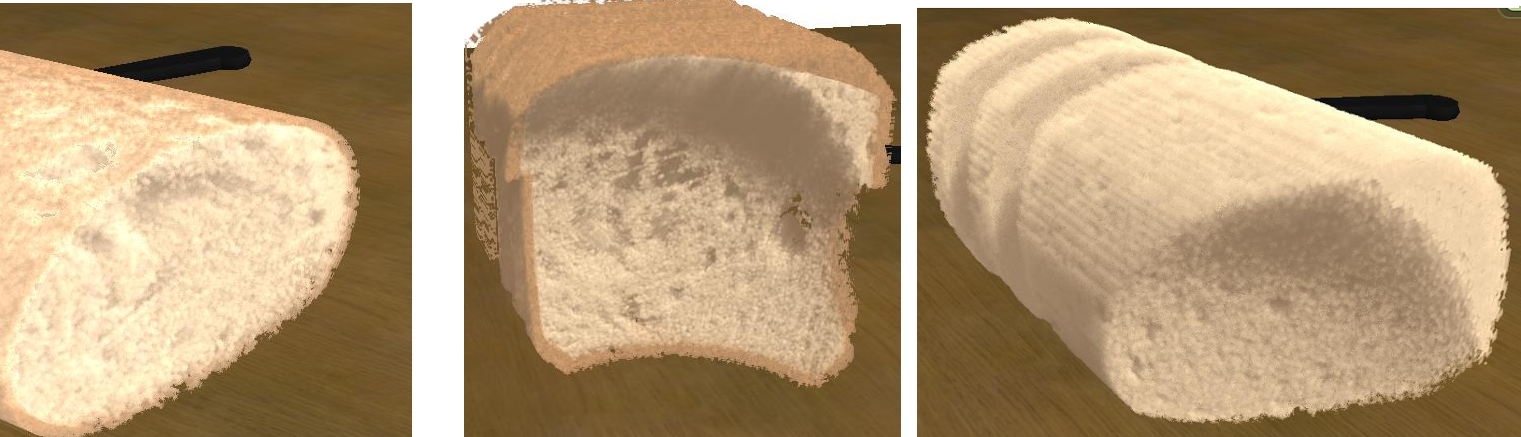
\includegraphics[scale=0.3]{fig5}}
  \caption{Different breads rendered in real time with the method described in this paper. The right image shows a bread which has no crust. }
  \label{fg:fig5}
\end{figure*}

Other materials could also be synthesised (see
Fig.~\ref{fg:fig6}). They are the result of varying different
parameters of the model. In the image, a sliced pudding (left) a slice
of cake (middle) and a sponge (right) are rendered. They have been
easily derived by changing the colour of the volume, and the structure,
in the case of the sponge. When no living yeast are involved in the
manufacturing process, a random volume texture could be used. Back
illumination is also present in the model (see Fig.~\ref{fg:fig7}). In
the figure, a sponge is illuminated from behind and light propagation
in its medium is seen.

\begin{figure*}[htb!]
  \centerline{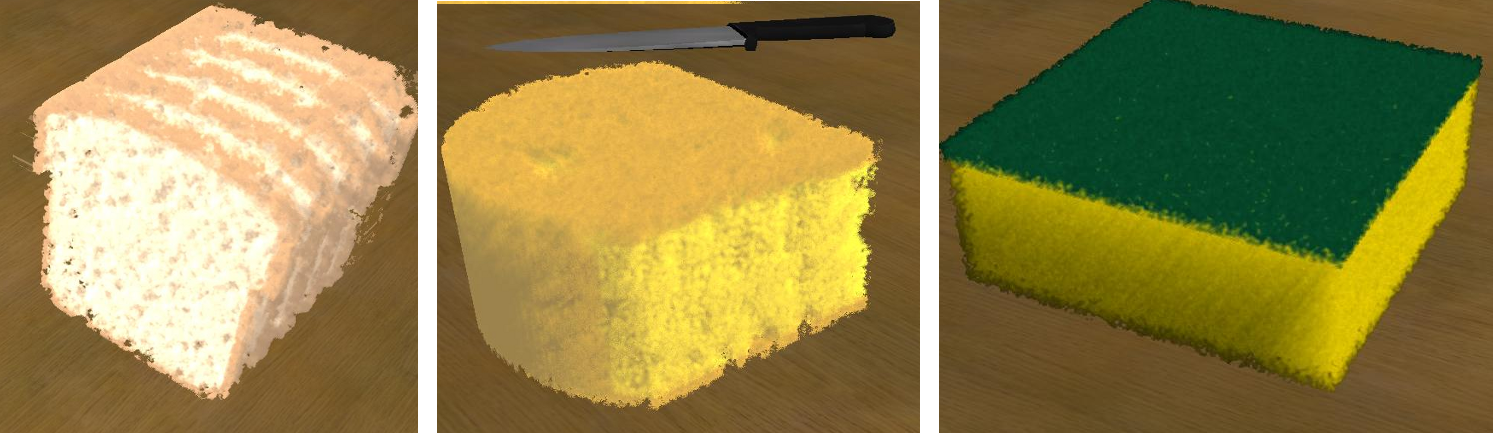
\includegraphics[scale=0.3]{fig6}}
  \caption{Other materials rendered in real time changing parameters in the model. Left: sliced pudding, middle: slice of cake, right: sponge. }
  \label{fg:fig6}
\end{figure*}



\begin{figure*}[htb!]
  \centerline{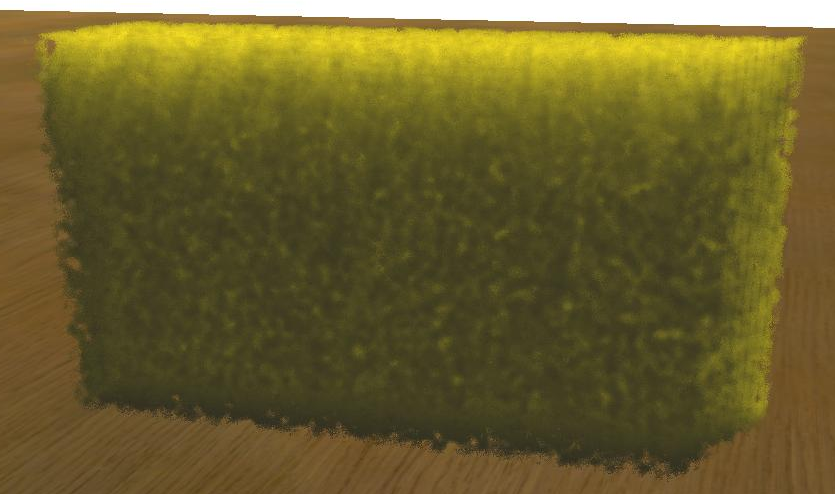
\includegraphics[scale=0.25]{fig7}}
  \caption{Sponge showing back illumination in the model. }
  \label{fg:fig7}
\end{figure*}


\subsection{Computing times}
Most images show real time results (FPS over 30), see Table~\ref{tab:n1} . The performance is affected mostly when the transmittance is low ({\em i.e.}, when the material becomes more transparent), since the ray accumulates more information (and the computation ends later). Another key parameter are the steps that a ray traverses. We experimentally found that values above $100$ steps give reasonably images in all cases. The process automatically scales with the number of GPU processors, so the fps count will increment in the GPUs of the next years.

\begin{table}[htb]
\centering
\begin{tabular}{|c|c|c|c|c|c|c|}
\hline &  Bread 1 & Bread 2 & Bread 3 & Pudding & Cake & Sponge \\
\hline
\hline
 mean FPS  & 32.2 &  75.5 &  45.2 & 28.5 &  54.2 & 29.7\\
\hline
 Steps &  140 &  140 &  140 & 256 &  140 & 256 \\
\hline
 Transmittance &  15 &  15 &  15 & 15 &  15 & 2.25 \\
\hline
\end{tabular}
\caption{Computing times and key parameters for the images obtained. }
\label{tab:n1}
\end{table}

\subsection{Discussion}
To the best of the authors knowledge, this is the first attempt to convincingly render bread crumb in real time without introducing complex intermediate processes (capture, mesh generation, precomputation, post-process). It is true that a previous approach \citep{Cho2007} has been used for bread rendering, but comparisons with this technique could not be established since no details are explained (computing times, render method).

Different regions with different parameters in the volume can be
defined, and this idea is used to show crumb and crust of different
colour parameters. 
%% Also, since entire regions of the volume could be
%%changed, the approach can be used in a simulation where a knife cuts
%%slices of bread. 
Integration with shader based engines is easily managed. Depth
information from fragments can be obtained, so it can be naturally
integrated in scenes, as the different images shows.

Computing times show an excellent performance which depends mostly on
the number of steps and the transmittance chosen. Nevertheless, real
time rates are always reached except when it encompasses a big portion
of the screen, since the approach is largely fragment-shader bound. In
years to come, this method will automatically augment its fps count
since it scales with the number of processors.

The promising results obtained can be extended in number of ways,
outlined at the end of this paper.


%\section{CONCLUSIONS AND FUTURE WORK}


%\subsection{Main headings}

%The main headings should be written left aligned, in 12pt, boldface
%and all capital Times Roman letters. There should be a 12pt space
%before, and 6pt after the main headings.

%\subsection{Secondary headings}

%The secondary headings should be written left aligned, in 12pt,
%boldface Times Roman, with an initial capital for first word only. There
%should be a 12pt space before, and 6pt after the secondary headings.

%\section{TEXT}

%The normal text should be written single-spaced, justified, using 12pt
%Times Roman in one column. The first line of each paragraph must be
%indented 0.5cm. There is not inter-paragraph spacing.

%\section{PAGE NUMBERS}

%The authors {\bf must not number} the pages of the article. Numbers will
%be added by the editor/publisher. 

%\section{FIGURES}

%All figures should be numbered consecutively and captioned. The
%caption should be written centered, in 10pt Times Roman, upper and lower
%case letters.

%\begin{figure*}[htb]
%\centerline{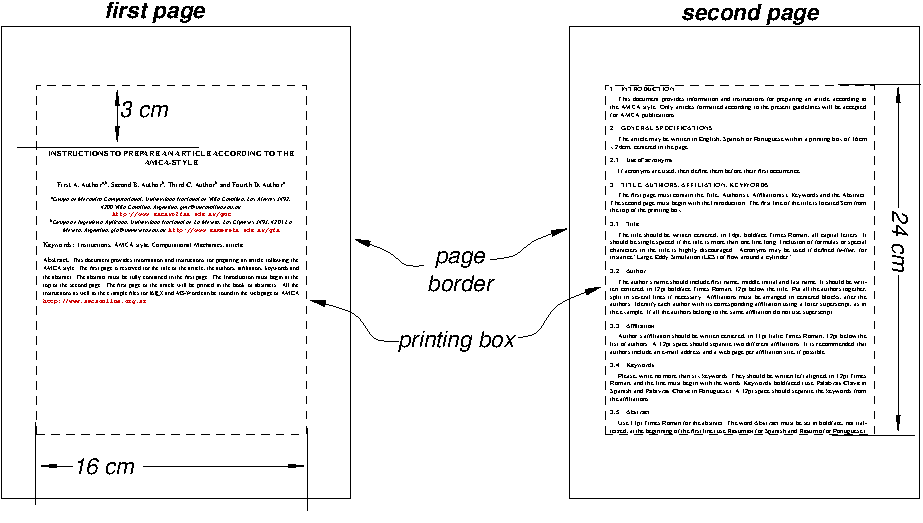
\includegraphics{firstpage}}
%\caption{Page layout}
%\label{fg:figure}
%\end{figure*}

%A 6pt space should separate the figure from the caption, and a
%12pt space should separate the upper part of the figure and the
%bottom of the caption from the surrounding text (see
%Fig.~\ref{fg:figure}).

%Figures should be referenced in the text. Color figures are welcomed.

%\section{EQUATIONS}

%A displayed equation is numbered, using Arabic numbers in parentheses.
%It should be  centered, leaving a 6pt space above and below to separate it from
%the surrounding text.

%The following example is a simple single line
%equation
%
%\begin{equation}
%Ax = b.
%\end{equation}

%The next example is a multi-line equation
%
%\begin{equation} \label{eq:simple}  
%\begin{aligned}
%Ax& = b,\\
%Ax& = c.
%\end{aligned}
%\end{equation}
%
%If possible, internal PDF links must be generated for references to
%equations. The recommended color for links to references in the text
%is blue (e.g., see Eq.~(\ref{eq:simple})).

%\section{TABLES}

%All tables should be numbered consecutively and captioned, the caption
%should be 10pt Times Roman, upper and lower case letters.

%A space of 6pt separates the table from the caption, and 12pt space
%separates the table from the surrounding text. For an example, see
%Table~\ref{tab:n50}. Tables should be referenced in the text.

%\begin{table}[htb]
%\centering
%\begin{tabular}{|c|c|c|c|}
%\hline  & 20x20 mesh & 50x50 mesh & 100x100 mesh\\
%\hline
%\hline
% 0 & 41.00 & 1.00 & 4.92\\
%\hline
% 1 & 40.86 & 1.02 & 4.88 \\
%\hline
%10 & 23.81 & 3.44 & 2.92 \\
%\hline
%50 & 5.62 & 64.20 & 1.08 \\
%\hline
%\end{tabular}
%\caption{Condition number for the Stekhlov operator. }
%\label{tab:n50}
%\end{table}

%\section{FORMAT OF REFERENCES}

%References should be quoted in the text using the \emph{author-style}
%(a.k.a. \emph{Harvard style}). References can be cited in
%\emph{parenthetical} form \citep{zienkiewicz91,idelsohn94,meyer82,meyer82b}, or
%in \emph{textual} form, e.g. see
%\citet{zienkiewicz91,idelsohn94,meyer82,meyer82b}.  References are grouped
%together and sorted alphabetically at the end of the article as shown
%in these instructions. Do not include references that are not cited in
%the article body. 

%If possible, internal PDF links must be generated for citations. The
%recommended color for links to references in the text is blue. The
%preferred color for links to external references, as web pages, 
%is red (e.g. \url{http://www.amcaonline.org.ar}).

\section{CONCLUSIONS}

In this paper the transmittance model of DVR is applied in the GPU to a 3D scalar field representing the bread crumb structure, to obtain realistic bread crumb images. This structure is generated using particle systems in which particles follow dynamical systems in a probabilistic way. A numerical simulation is employed to solve the resulting set of equations which represents the dynamical system. Results show high fidelity images in real time, suitable for application in several areas, such as serious games \citep{Susi2007} and photo-realistic rendering. This procedure does not present the drawbacks of other state of the art methods, such as capture processes or mesh generation.

The main disadvantage of the method is resolution, since close look-ups of the structure could lead to homogeneous areas due to hardware constraints, {\em i.e.}, arbitrary texture sizes are not allowed. This disadvantage is not exclusive of our method. A number of possible solutions will be employed to overcome this problem, such as setting different volume textures depending on the distance to the volume. 

As possible continuations of this work, DVR could be extended to handle other phenomena such as indirect illumination and sub surface scattering in order to enhance the images obtained. Also, partial differential equations will be employed to implement the baking process of bread \citep{Purlis2012}. Other porous materials such as cheeses will be investigated. Another interesting work will be to define primitives for crumb and crust modelling (shapes and intersections), enabling artists to define its shape.

%Template files in TeX, \LaTeX{} and MS-Word may be found at the
%AMCA web site: \url{http://www.amcaonline.org.ar}. 
%Remember: {\bf Do not number the pages.}
%
\bibliography{eniefbib}
\end{document}
% $Id: amcapaper.tex,v 1.23 2006/08/14 16:58:45 mstorti Exp $
